\documentclass[handout]{beamer}
\usepackage[frenchb]{babel}
\usepackage[T1]{fontenc}
\usepackage[utf8]{inputenc}
\usepackage{graphicx}


% functions to plot
\def\func(#1){(#1)*(1-(#1))}
\hypersetup{colorlinks = true,linkcolor = blue,urlcolor  = blue}
            
\newcommand{\qGraph}[1]{\begin{center} \includegraphics[width =
\textwidth]{#1}\end{center}}

\newcommand{\mcl}{\mathcal}


\newenvironment{iPar}[1]{\textbf{#1} \begin{itemize}}{\end{itemize}}

\newcommand{\inc}{{inc}}
\newcommand{\cp}{{cmp}}
\newcommand{\bull}{$\bullet\;$} 

\newcommand{\esp}{\mathbf{E}} \newcommand{\ul}[1]{\underline{#1}}
\newcommand{\ol}[1]{\overline{#1}} \newcommand{\ora}[1]{\textbf{#1}}
\newcommand{\wh}{\widehat}
\newcommand{\mdp}{\medskip \pause}
\newcommand{\mc}{\mathcal}

\title{Exchange Economy and Price Signals}
\author{Microeconomics \\ 20851}
\date{}

\begin{document}

\frame{\titlepage}

\section[Outline]{}
\frame{\tableofcontents}

\section{}


\begin{frame}\frametitle{Roadmap}

\begin{iPar}{Up until now}
\item Consumer choice
\item Price and income effects
\item Risk and time
\item Measuring welfare and well-being
\end{iPar}\mdp

\begin{iPar}{This class: Exchanges}
\item Market equilibrium in an exchange economy
\end{iPar}\mdp

\begin{iPar}{Coming up}
\item  Production decisions in firms
\item Strategic behaviour of firms
\item Auctions
\end{iPar}


\end{frame}

\section{Market equilibrium}

\begin{frame}\frametitle{Exchange Economy}

\begin{iPar}{Context} \item Consider a situation with two consumers (1 and 2) and two goods ($X$ and $Y$) \item Utility fuctions $U_1(X,Y)$ and
$U_2(X,Y)$ \item Each consumer has an endowment of each good, $B_1^e = (X_1^e,Y_1^e)$ and $B_2^e = (X_2^e,Y_2^e)$. \end{iPar}
\mdp


\begin{iPar}{Examples} \item 2 farmers, one has an endowment of potatoes and the other has an endowment of livestock. \item  Two countries: Country 1 has a petroleum endowment and Country 2 has a machinery endowment \item Where do these endowments come from? Nature (resources) or production
(consumer goods, machinery ...). We will talk about this further in the "Production" class. 
\end{iPar}

\end{frame}

\begin{frame}\frametitle{Market Equilibrium}

\begin{iPar}{Individual demand} \item Consumer 1 choses to consume $(X_1^c, Y_1^c)$  \item Given the prices $p_X$ and $p_Y$, the budget constraint is $$  p_X X_1^c + p_Y Y_1^c  =  p_X X_1^e + p_Y Y_1^e$$
\item Prices will be determined in equilibrium.
\end{iPar}\mdp

\begin{iPar}{Normalization}
\item  Two unknown prices $p_X$ and $p_Y$. Only relative price matters: the budget constraint can be written as follows : $$
X_1^c + \frac{p_Y}{p_X} Y_1^c  =   X_1^e + \frac{p_Y}{p_X} Y_1^e$$
\item Let's define the relative price as  $p = p_Y/p_X$  \end{iPar}
\end{frame}

\begin{frame} \frametitle{Market Equilibrium -- II}

\begin{iPar}{Definition} \item Individual demand:  $ \max U_1$ subject to  $ X_1^c + p Y_1^c  =   X_1^e + p Y_1^e$
\item We obtain $X_1^c(p)$ and $Y_1^c(p)$
\item  $p^*$ is an equilibrium price only if at
$p^*$ demand is equal to supply $$X_1^c(p^*)+X_2^c(p^*) = X_1^e + X_2^e \quad
and \quad Y_1^c(p^*)+Y_2^c(p^*) = Y_1^e + Y_2^e  $$ \item $X_1^c(p^*) -
X_1^e =X_2^e - X_2^c(p^*)  \;$  is the amount of $X$ that is exchanged  \item si $X_1^c - X_1^e < 0$, consumer 1 is a net supplier of $X$.\end{iPar}\end{frame}


\begin{frame}{Important Assumptions}
\begin{itemize} \item Competitive market:
consumers are  \textbf{price takers} \item All sold goods are homogeneous (identical) and percieved the same way by both the buyer and the seller \item The utility of consumer 1 does not depend on the actions of the other consumer: \textbf{no externalities} \end{itemize} \end{frame}



\begin{frame}\frametitle{An Example} \begin{iPar}{Context}\item $U_1(X,Y) =
U_2(X,Y) = \log X + \alpha \log Y$ \item Price $p_X= 1$, $p_Y = p$.
\item Endowment $X_1^e, Y_1^e, X_2^e, Y_2^e$ \end{iPar} \mdp
\begin{iPar}{Equilibrium} \item Solution of individual demands: $$X_1^c =
\frac{1}{1+\alpha}(X_1^e + p Y_1^e) \quad and \quad Y_1^c =
\frac{\alpha}{1+\alpha}\frac{X_1^e + p Y_1^e}{p} $$ \item Market equilibrium for $X$  \begin{equation*} X_1^c(p) + X_2^c(p) = X_1^e + X_2^e
\Rightarrow p = \alpha \frac{X_1^e + X_2^e}{Y_1^e + Y_2^e}
 \end{equation*} \item Notice that the market for $Y$ has also reached an equilibrium at $p$.\\\pause \textbf{Question:} only one unkown variable and two equations?\end{iPar} \end{frame}

\begin{frame} \frametitle{Walras' Law}

\begin{iPar}{One unkown variable but two equations} \item No problem: equilibrium on one market implies equilibrium on the other \item Budget constraint: $$ X_1^c + p Y_1^c  =   X_1^e + p Y_1^e \quad and \quad
X_2^c + p Y_2^c  =   X_2^e + p Y_2^e$$ \pause If we add one constraint to the other $$ [X_1^c + X_2^c] + p [Y_1^c + Y_2^c] = [X_1^e + X_2^e] + p
[Y_1^e + Y_2^e]$$ \pause An equilibrium in $X$  implies $$ p
[Y_1^c + Y_2^c]  = p [Y_1^e + Y_2^e] \Rightarrow  Y_1^c + Y_2^c = Y_1^e +
Y_2^e$$ \end{iPar}

\end{frame}

\begin{frame}\frametitle{What determines the price?}

\begin{iPar}{Compared static} \item How $p$ varies with $\alpha$
(importance of the good $Y$) and the aggregated quantities of $X$ and $Y$ ?
\pause \item If $\alpha$ $\nearrow$ then $p=p_Y$ $\nearrow$: since the total supply of $Y$ is fixed, when demand for $Y$ increases, the price must adjust to maintain the equilibrium. \pause \item If $Y_1^e + Y_2^e
\nearrow$ then $p=p_Y$ $\searrow$: the price must fall to sell the endowment. 
\pause \item If $X_1^e + X_2^e \nearrow$ then $p = p_Y$ $\nearrow$ since $Y$ has become rarer relative to $X$\end{iPar}

\end{frame}

\section{Pareto-efficient allocation}

\begin{frame}\frametitle{The Edgeworth Box} 

\begin{itemize}
    \item We draw the space of possible allocations in an Edgeworth box
    \item The initial endowment is a point in this space
\end{itemize}
 
\textbf{Exercise A}: Show the endowment $(x^e_1,y_1^e) = (50,20)$ and $(x^e_2,y_2^e)=(20,50)$ in an Edgeworth box.
\end{frame}


\begin{frame}\frametitle{Pareto-Efficient Allocation}
\begin{itemize}
    \item A point on the Edgeworth box where indifference curves cross is not Pareto-optimal. 
    \item We can define the core of this point as all the allocations that are a Pareto improvement. 
    \item When the core is empty, we get an allocation that is Pareto-efficient : this implies that the indifference curves are tangent.
    \item The Pareto Frontier (or Pareto Front) is the curve that shows all the allocations that are Pareto-efficient. 
\end{itemize}

\end{frame}

\begin{frame}{Calculating an optimum}

We can seek to maximize the welfare of an agent by keeping the other's fixed and respecting the resource constraints: 

\begin{eqnarray*}
\max_{X_1,Y_1,X_2,Y_2} u(X_1,Y_1) 
\end{eqnarray*}
subject to:
\begin{eqnarray*}
u(X_2,Y_2)\ge \overline{u}_2 \\
X_1 + X_2 \le X_e \\
Y_1 + Y_2 \le Y_e
\end{eqnarray*}

\end{frame}

\begin{frame}\frametitle{A Few Exercises} 


\textbf{Exercise B}: Find the Pareto-optimal allocation for the utility functions $u_1$ and $u_2$ strictly positive and concave, $u_j = \sqrt{x_j y_j}$ for consumers $j=1,2$, using the Lagrangian method.

\textbf{Exercise C}: Find the Pareto-optimal allocation for the utility functions $u_j = \sqrt{x_j y_j}$ for consumers $j=1,2$ with the total endowments $x_e = 128$ and $y_e=32$ if $\overline{u}_2=48$.

\textbf{Exercise D}: In Exercise C, is the allocation $(64,28,64,4)$ optimal? If it isn't, find a Pareto improvement that can be made in the core. 

\end{frame}

\begin{frame}{Market Equilibrium in an Edgeworth box}
\begin{itemize}
    \item The budget constraint is given by the endowments and indicates which allocations are possible at price $p$. 
    \item A market equilibrium implies that the $MRS$ are equal to the price ratio.
\end{itemize}
\end{frame}

\begin{frame}\frametitle{Exchange is Better Than Autarky}

\begin{iPar}{Property:} \item Consider the equilibrium price: $p^*$ and the quantities consumed by consumer 1: $X^c_1 = X^c_1(p^*)$ and $Y^c_1 = Y^c_1(p^*)$ \item We have $U_1(X^c_1, Y^c_1) \geq U_1(X^e_1, Y^e_1)$
\end{iPar}\mdp

\begin{iPar}{Why?} \item At $p^*$, the basket $B^e_1 = (X^e_1,Y^e_1)$ is available and consumer 1 chooses $B^c_1=(X^c_1, Y^c_1)$ \item This implies that $U_1(X^c_1, Y^c_1) \geq U_1(X^e_1, Y^e_1)$
\pause \item Note: If $U$ concave and $(X^c_1, Y^c_1) \neq (X^e_1,
Y^e_1)$ then $U_1(X^c_1, Y^c_1) > U_1(X^e_1, Y^e_1)$ \end{iPar}

\end{frame}

\section{Welfare theorems}

\begin{frame}\frametitle{Propeties of a Market Equilibrium (I) -- 1st Theorem of Welfare} \begin{iPar}{1st theorem of welfare} \item  A market equilibrium is always Pareto-optimal. \item 
In an allocation that is Pareto-efficient we cannot make a consumer better off without making another consumer worse off \end{iPar}\mdp



\begin{iPar}{Why?} \item<1-> At the equilibrium allocation
$X^c_1(p^*),Y^c_1(p^*),X^c_2(p^*),Y^c_1(p^*)$ the indifference curve of consumer 1 is tangent to the budget constraint, and tangent to the indifference curve of consumer 2 \item<2-> This implies that the allocation is Pareto-efficient.\end{iPar}

\end{frame}


\begin{frame}\frametitle{The 2nd Theorem}

\begin{iPar}{The 2nd theorem of welfare} \item We can achieve any Pareto-efficient allocation we desire through market equilibrium if we redistribute the initial endowments \item This requires the ability to impose taxes (lump-sum payments) \item Often called a decentralized resource allocation
\end{iPar}\mdp

\begin{iPar}{Why?}\item Suppose there's no corner solution \item At any allocation $(X_1^*,Y_1^*)$ (and consequent value for
$X_2^*,Y_2^*$) the indifference curve of the two consumers are tangent.
\item Consider this tangence line. \item Any of the allocations on that line results in a market equilibrium  $(X^*,Y^*)$. \end{iPar}

\textbf{Exercise E}: Find the endowment transfer and the price, starting from $(64,28,64,4)$, which give the optimal allocation found in D.  

\end{frame}


\begin{frame}\frametitle{Market Efficiency}
\begin{iPar}{The 1st and 2nd theorems establish that} \item
The market is efficient \item If for one reason or another we want another allocation, we can achieve it by redistributing the resources and letting the market take its course  \end{iPar}\mdp

\begin{iPar}{An important result: Decentralized efficiency} \item A market equilibrium requires only that agents know their own preferences   \item There is no need for a central planner that knows everyone's preferences \item We naturally obtain a Pareto-efficient result \item
Hayek's take: markets are information aggregators \item Planned economies lose this information (not to mention that it is costly to find  preferences of every citizen). 
\end{iPar}

\end{frame}

\begin{frame}\frametitle{Epilogue -- II -- limits}

\begin{iPar}{These two theorems are interesting, but they rest on important hypotheses} 
\item Competitive markets (price takers) \item Goods are homogeneous (we know what we're buying) \item No externalities
\item We can impose lump-sum taxes (for the 2nd theorem)\end{iPar}\mdp

The general equilibrium theory had quite an impact on economics: think about how we understand financial markets or macroeconomics. 

\end{frame}

\section{A bit of history}

\begin{frame}\frametitle{History of the General Equilibrium Theory}

\begin{figure}
\centering
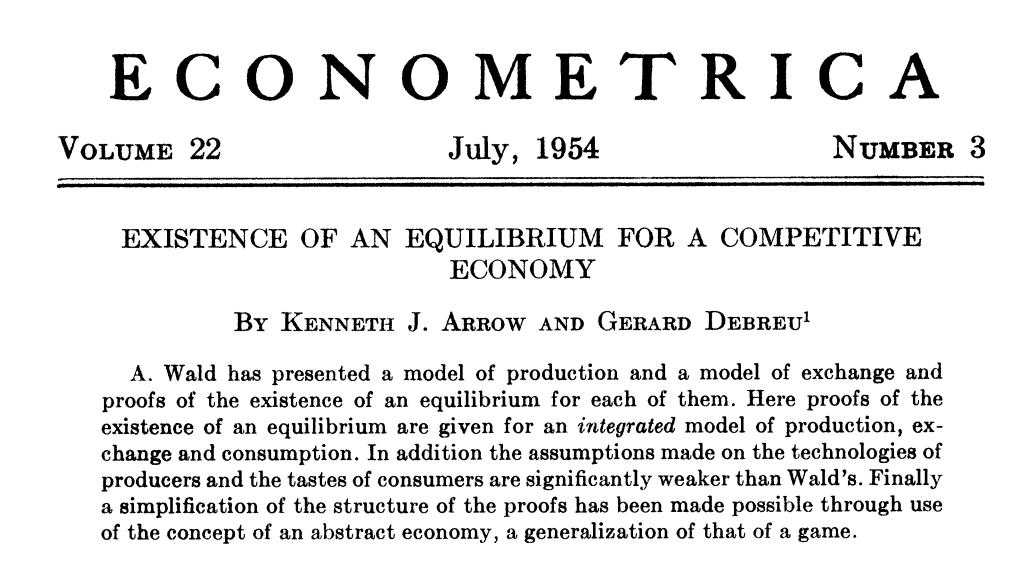
\includegraphics[scale=0.5]{ad1954.png}
\end{figure}

\end{frame}


\begin{frame}\frametitle{History of the General Equilibrium Theory}

They came from very different backgrounds (Arrow, economics), (Debreu, mathematics). Düppe (2017) tells the story of how this project came to be.  

\begin{figure}
\centering

\includegraphics[scale=0.35]{invitation.png}
\caption{\href{https://www.cambridge.org/core/journals/journal-of-the-history-of-economic-thought/article/div-classtitlearrow-and-debreu-de-homogenizeddiv/761E76D5A52C948615066F502277D9DD}{Duppe (2017), Journal of History of Economic Thought}}
\end{figure}

\end{frame}

\end{document}




